%!TEX root = ../Thesis.tex

\chapter{Prototype}
The Ground Control Platform must have some physical dimension due to the size of the UAV used in this project. The dimension of the UAV used will affect the dimension and choice of construction of the ground station. In dimensioning and designing the ground station the primary focus is on making an industrial and robust prototype. 



\section{Landing platform / Helipad}
The landing platform or helipad is a 60cm x 60cm wide plate with a hole in the middle. Dimensioning of the size mainly relies on tolerance on the precision of landing the UAV. The UAV only needs 30cm x 30cm space for the landing gear, but in case a big wind gust comes in just before landing/take-off, the UAV can slide off the platform if the platform is too small. On figure \ref{fig:helipad} the helipad is seen from the top.

\begin{figure}[hbtp]
\centering
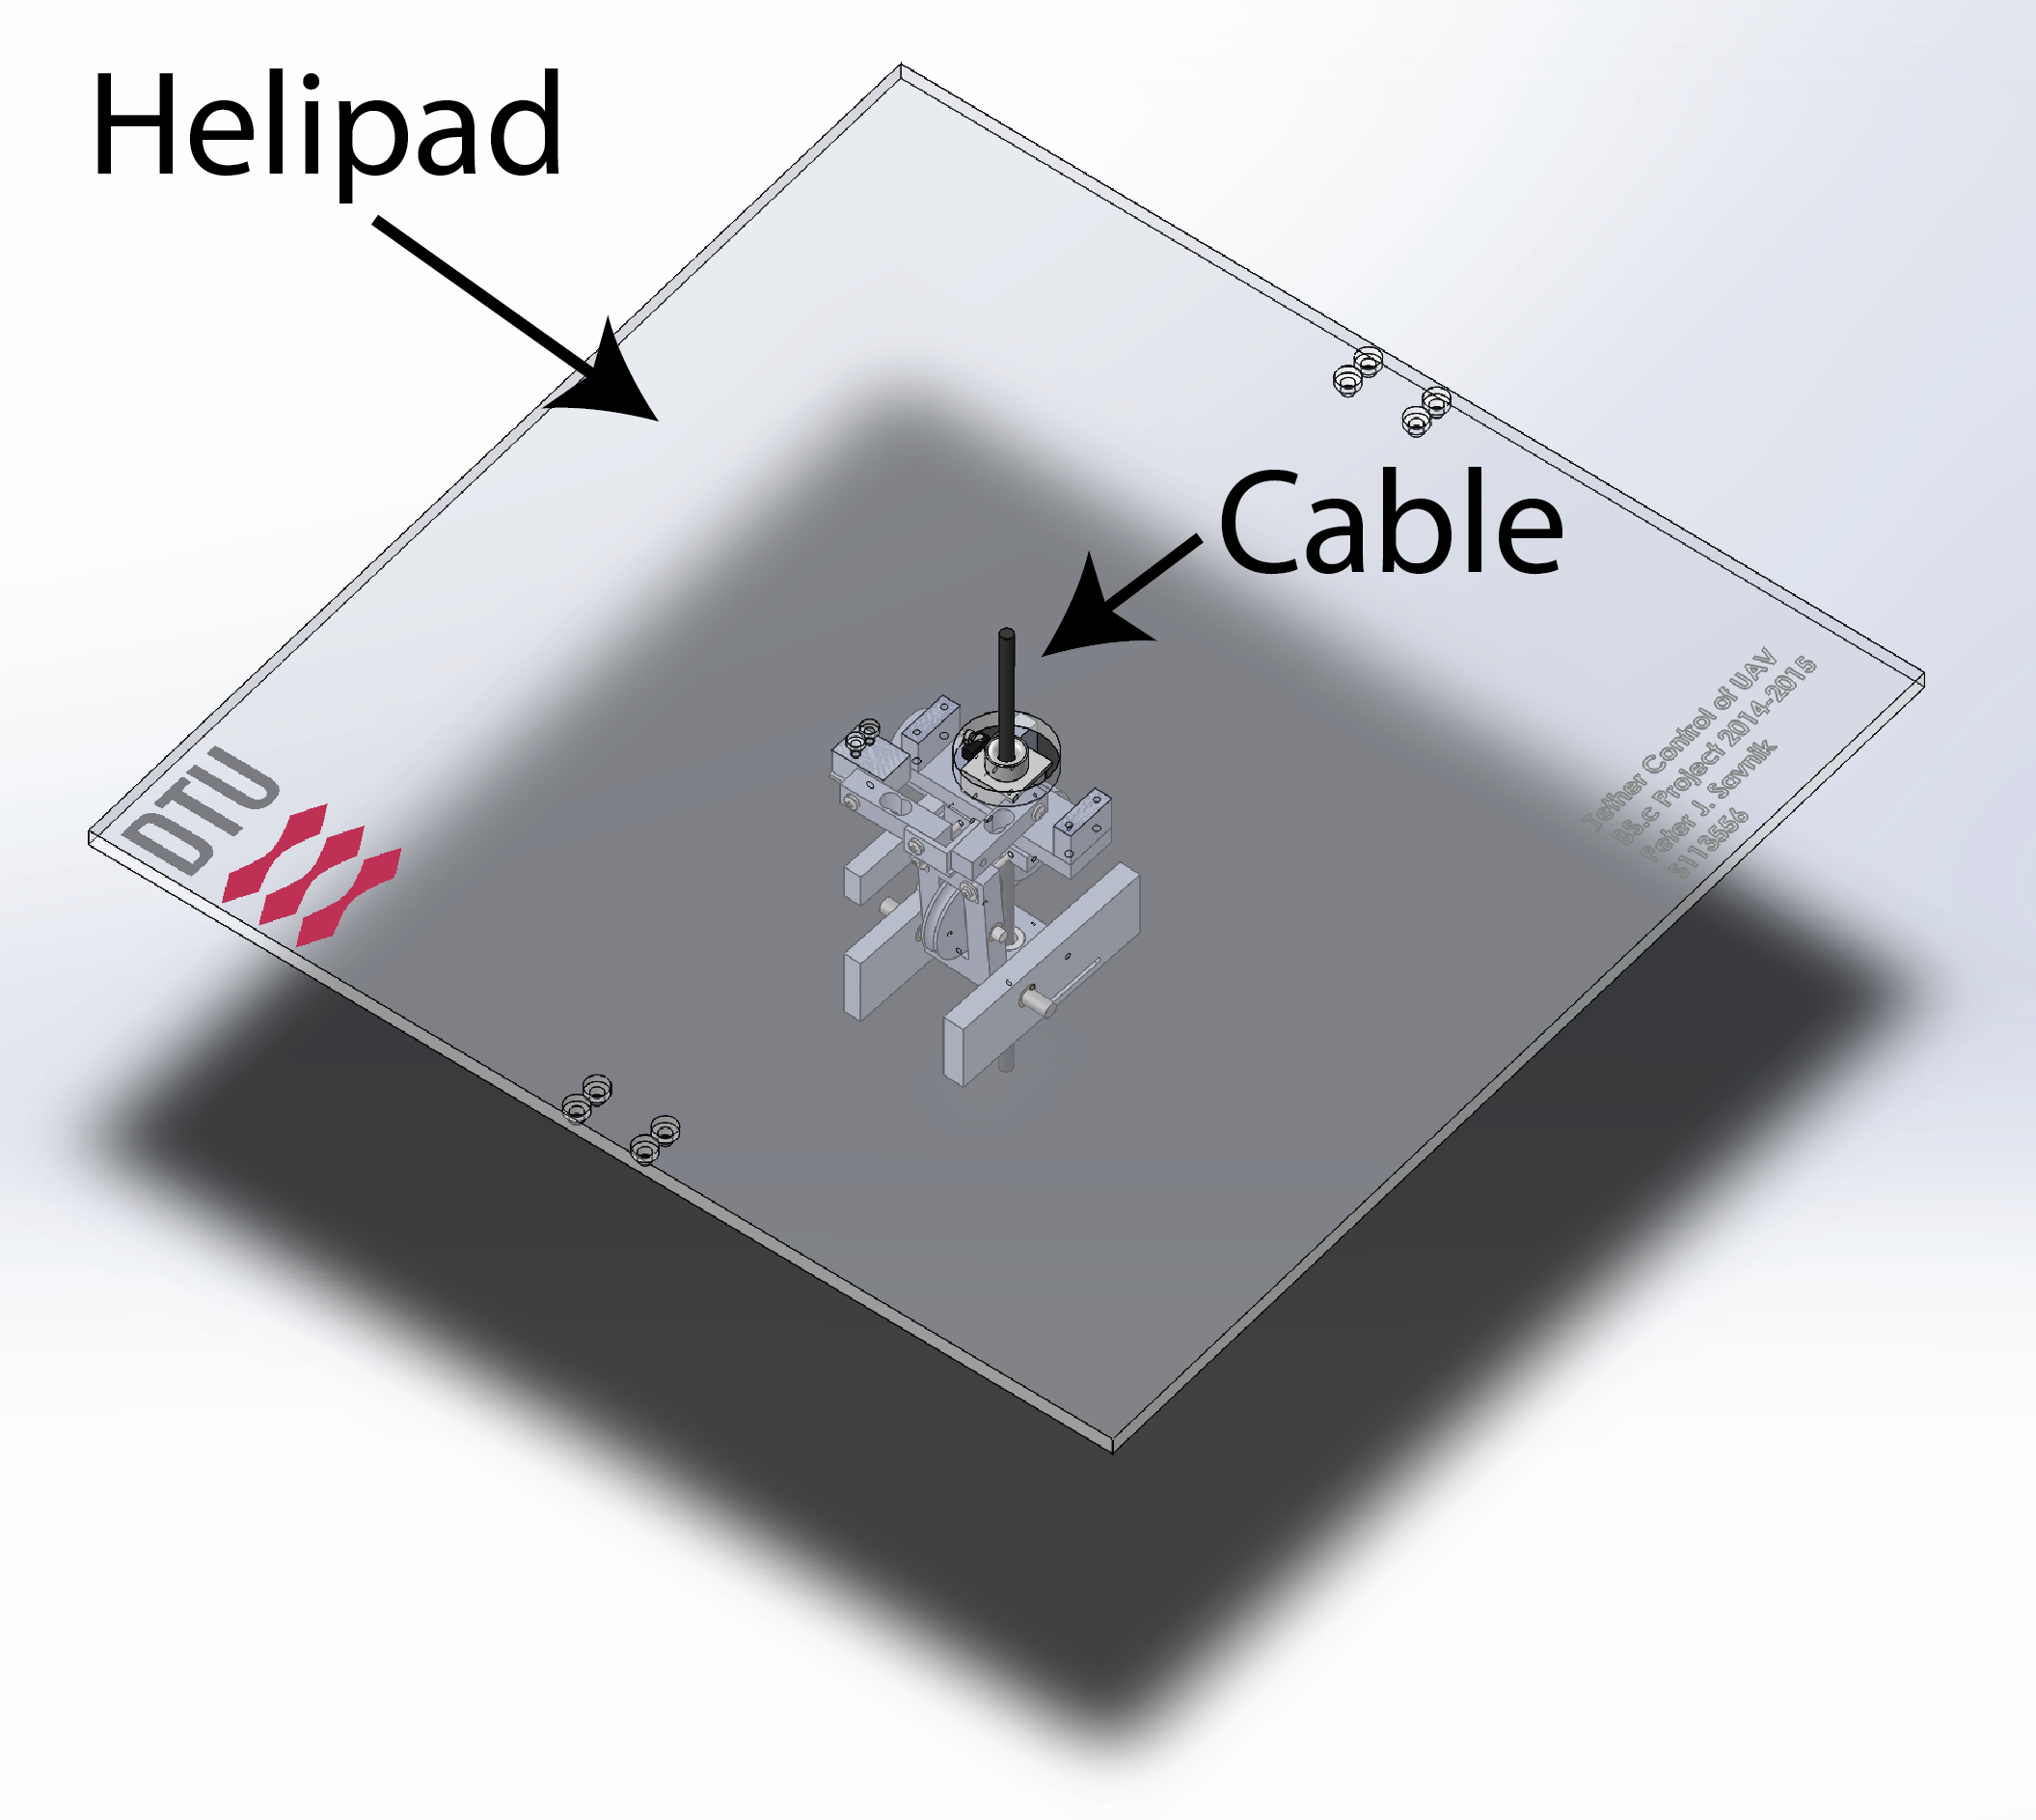
\includegraphics[scale=0.6]{graphics/cad/toplevel.png}
\caption{Illustration of Helipad with a hole in the middle for the cable.}
\label{fig:helipad}
\end{figure}

\section{Messuring the horisontal angle}
\label{sec:horizontalAnglePrototype}
In order to precisely determinate where the UAV is positioned relative to the helipad on a horizontal plane a coordinate system on figure \ref{fig:top-coordinates} is introduced. $x$ and $y$ are Cartesian coordinates corresponding to the measurements of load cell 1 and load cell 2 from figure \ref{fig:loadcells}. $\phi$ is the angle, starting at the positive $x$ direction and increases in positive direction of rotation.

\begin{figure}[hbtp]
\centering
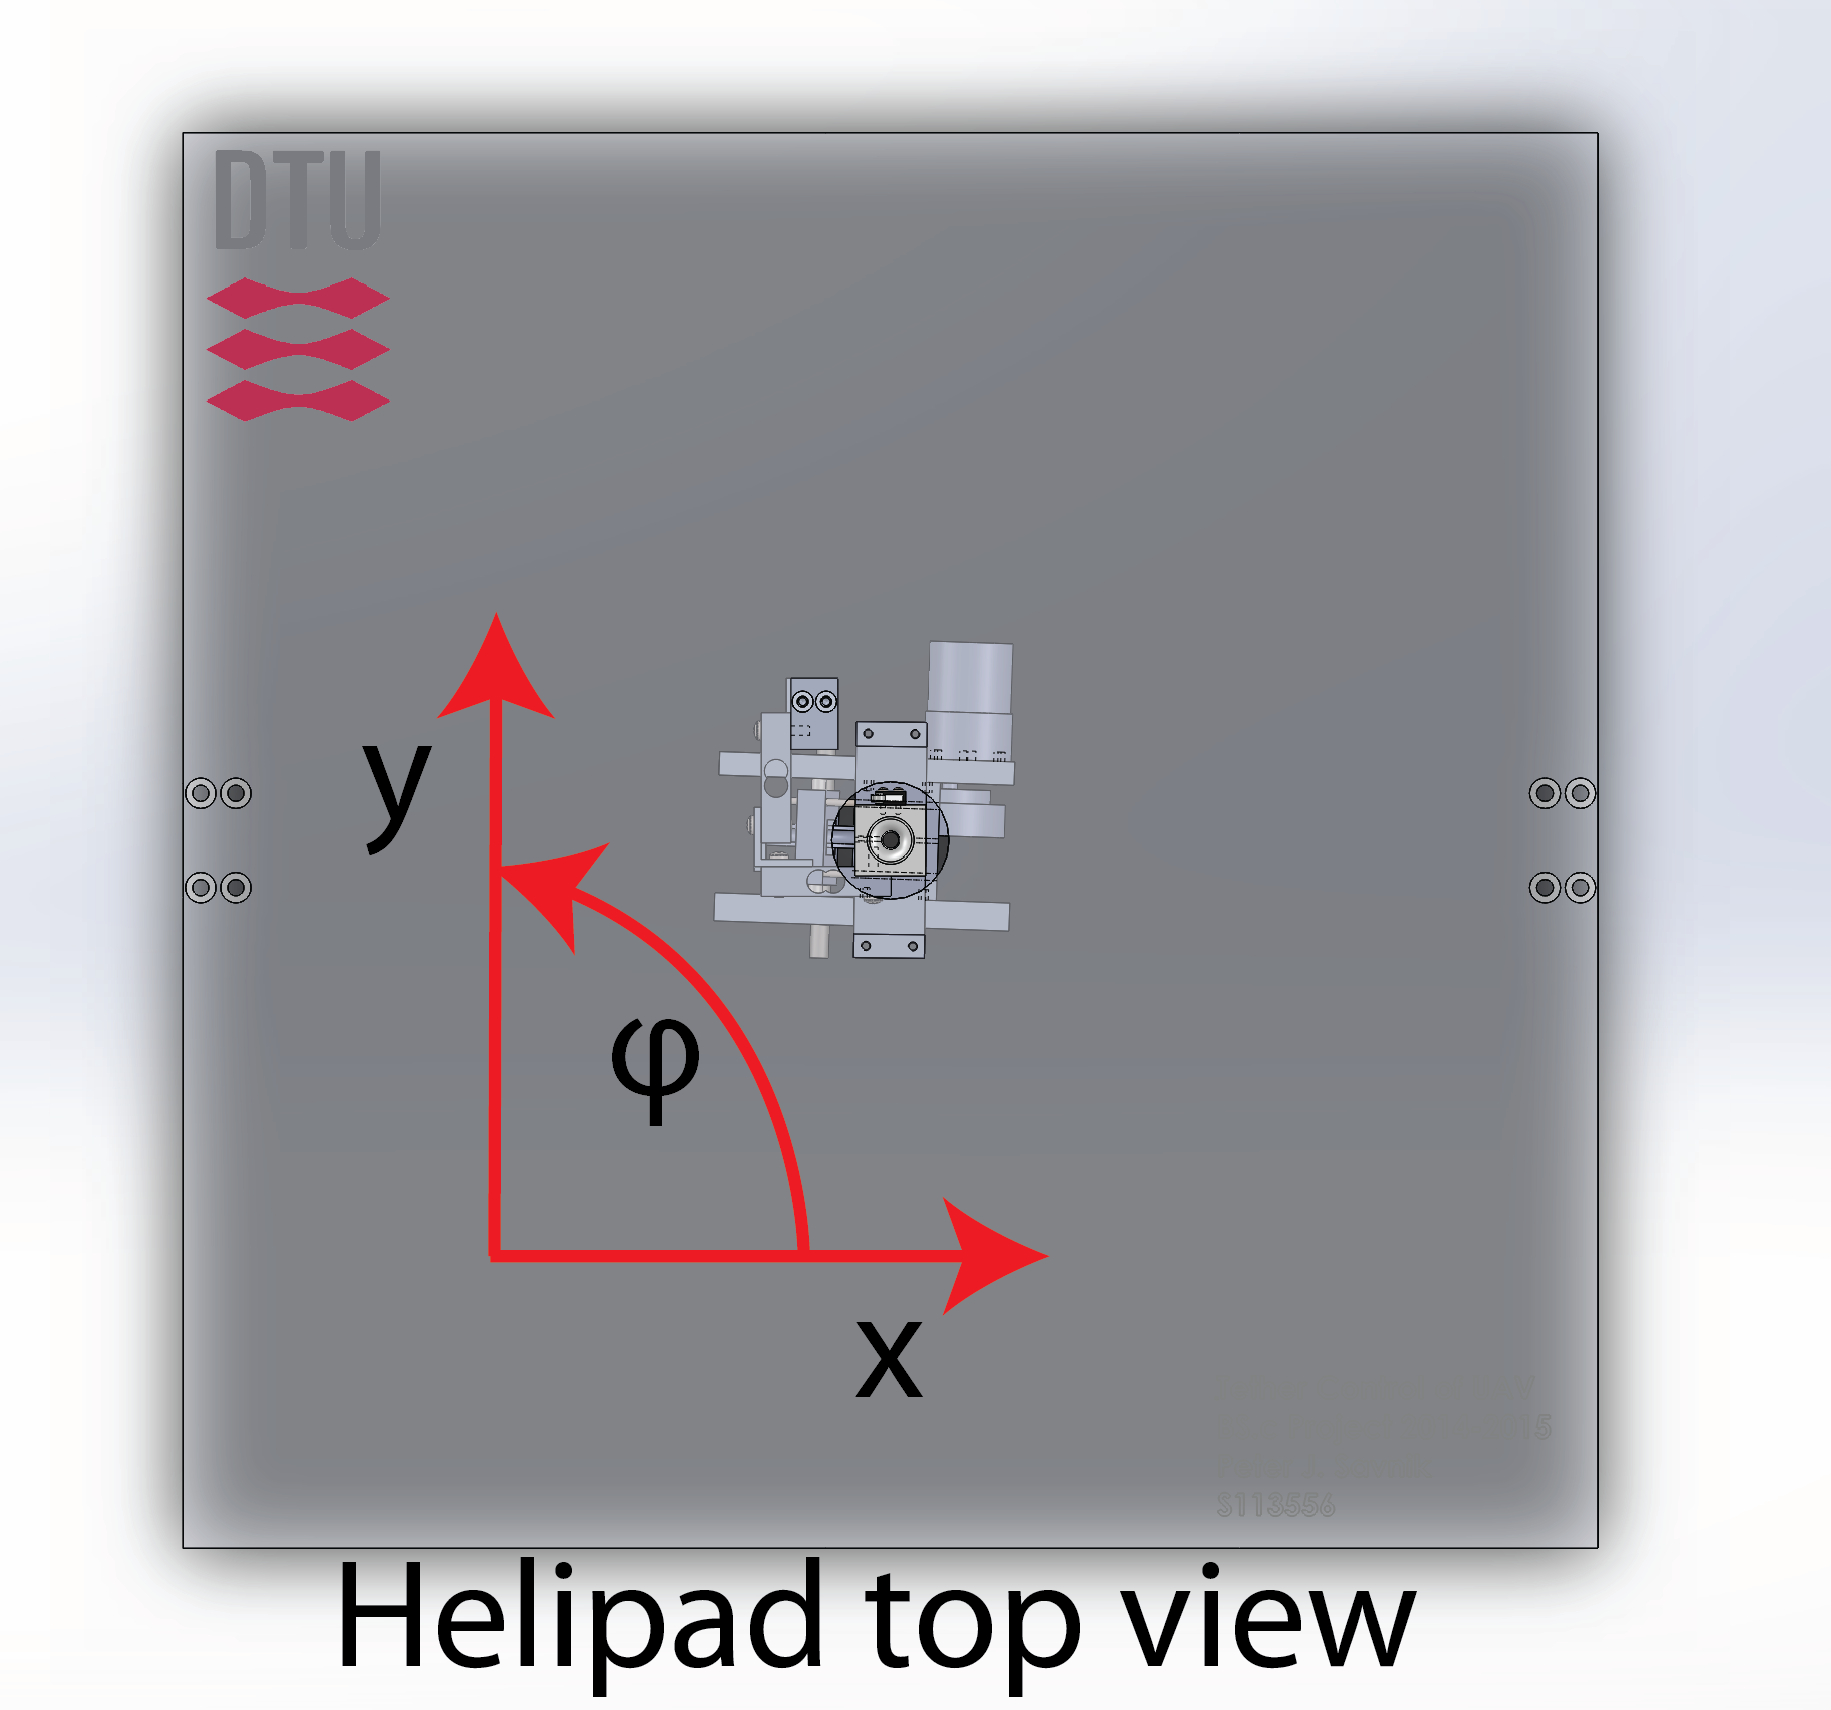
\includegraphics[scale=0.6]{graphics/cad/top-coordinates.png}
\caption{Helipad seen from top view with coordinate system.}
\label{fig:top-coordinates}
\end{figure}

\noindent
To measure the horizontal angle between the Ground Station and the UAV to load cells are used, perpendicular to each other. One end attached to the Ground Station and the other end attached to a cable though hole made in Teflon. Then the UAV is exactly direct over the centre, no force will be measured, but then the UAV moves to one of the sides it will create a cable tension that results in a force in $x$- and $y$-direction. Combining the $x$ and $y$ force can be translated to an angle. 

\begin{figure}[hbtp]
\centering
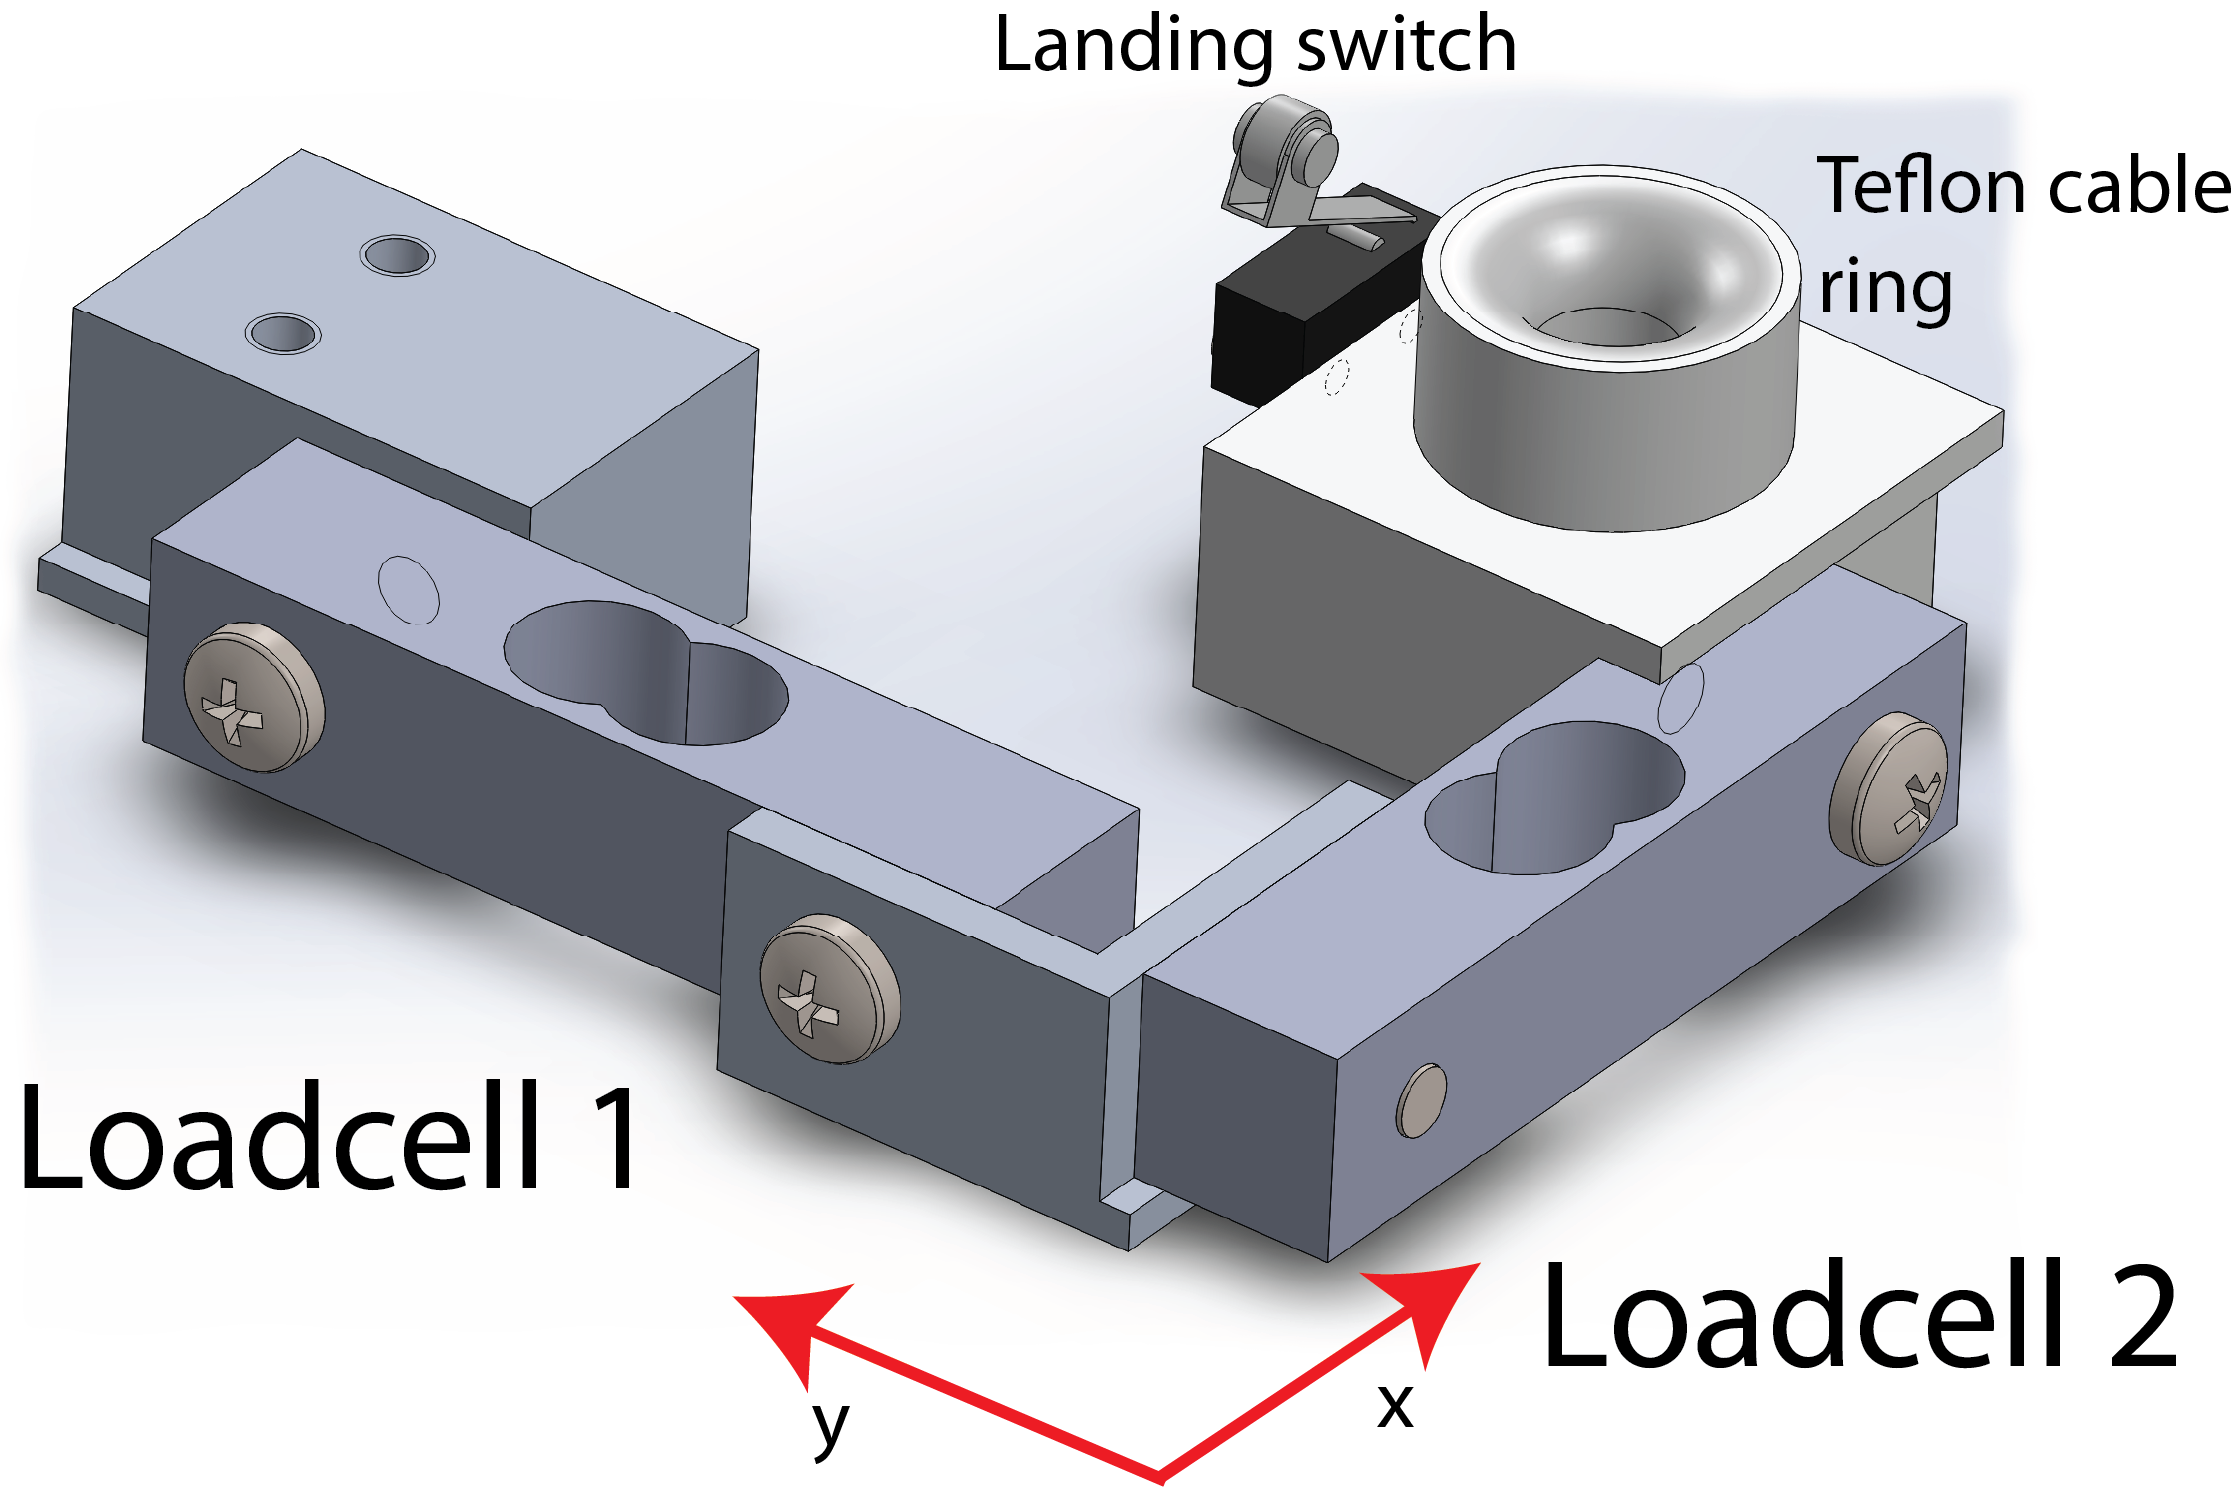
\includegraphics[scale=0.75]{graphics/cad/loadcell.png}
\caption[Configuration of two load cells, for measuring the cable drag]{Configuration of two load cells, for measuring the cable drag in x and y direction. Load cell 1 measures in $x$-direction and load cell 2 in $y$-direction.}
\label{fig:loadcells}
\end{figure}

\noindent
The UAV can lift about 3kg payload and therefore exert 3kg thrust to the cable and the measuring device must be able to withstand such a force without permanently bending. Two 5kg load cells from Phidget Inc is assessed to be the best match for the job with regard to what is available in the projects price range.








\section{Winching and storing the cable}
There are several ways to keep the cable when it's not rolled out, two commonly used methods are on a cable drum or in a winded pile. The critical parameters here is the flexibility of the cable, diameter of the cable and heat tolerances.  Because the cable is stored tightly together, heating from the cable resistance has to be given a thought in the cable storing design.

\subsection{Storing cable on a drum}
Storing cable on a drum is a very practical and commonly known method to store cables in a organised way. The benefits of this design is that the drum it self can be used as a winch to winch in the cable. But the minimum diameter of the drum is given by the cable minimum bending radius for flexible installation and that sets a physical minimum for the drums outer diameter. The larger the diameter the greater the force needed for rotating the drum. To assure smooth windings the drum can move from side to side. 
%Due to physics the movement from side to side will come natural, if the friction is low enough; in practise this concept works often but is not robust and that is why motorized guidance is needed\todo{referance}. 
In theory the rotation of the drum can be used as a feedback for how much cable is rolled out, but in practice this will be a source to a large margin of error. Further more this design is very dependent on the cable always have tension on. If there is no or too little tension on the cable it will loosen from the drum resulting is bad windings and the possibility for jams. \\
On figure \ref{fig:cable-drum} a cable drum is put under the helipad and the horizontal measurement device. 

\begin{figure}[H]
\centering
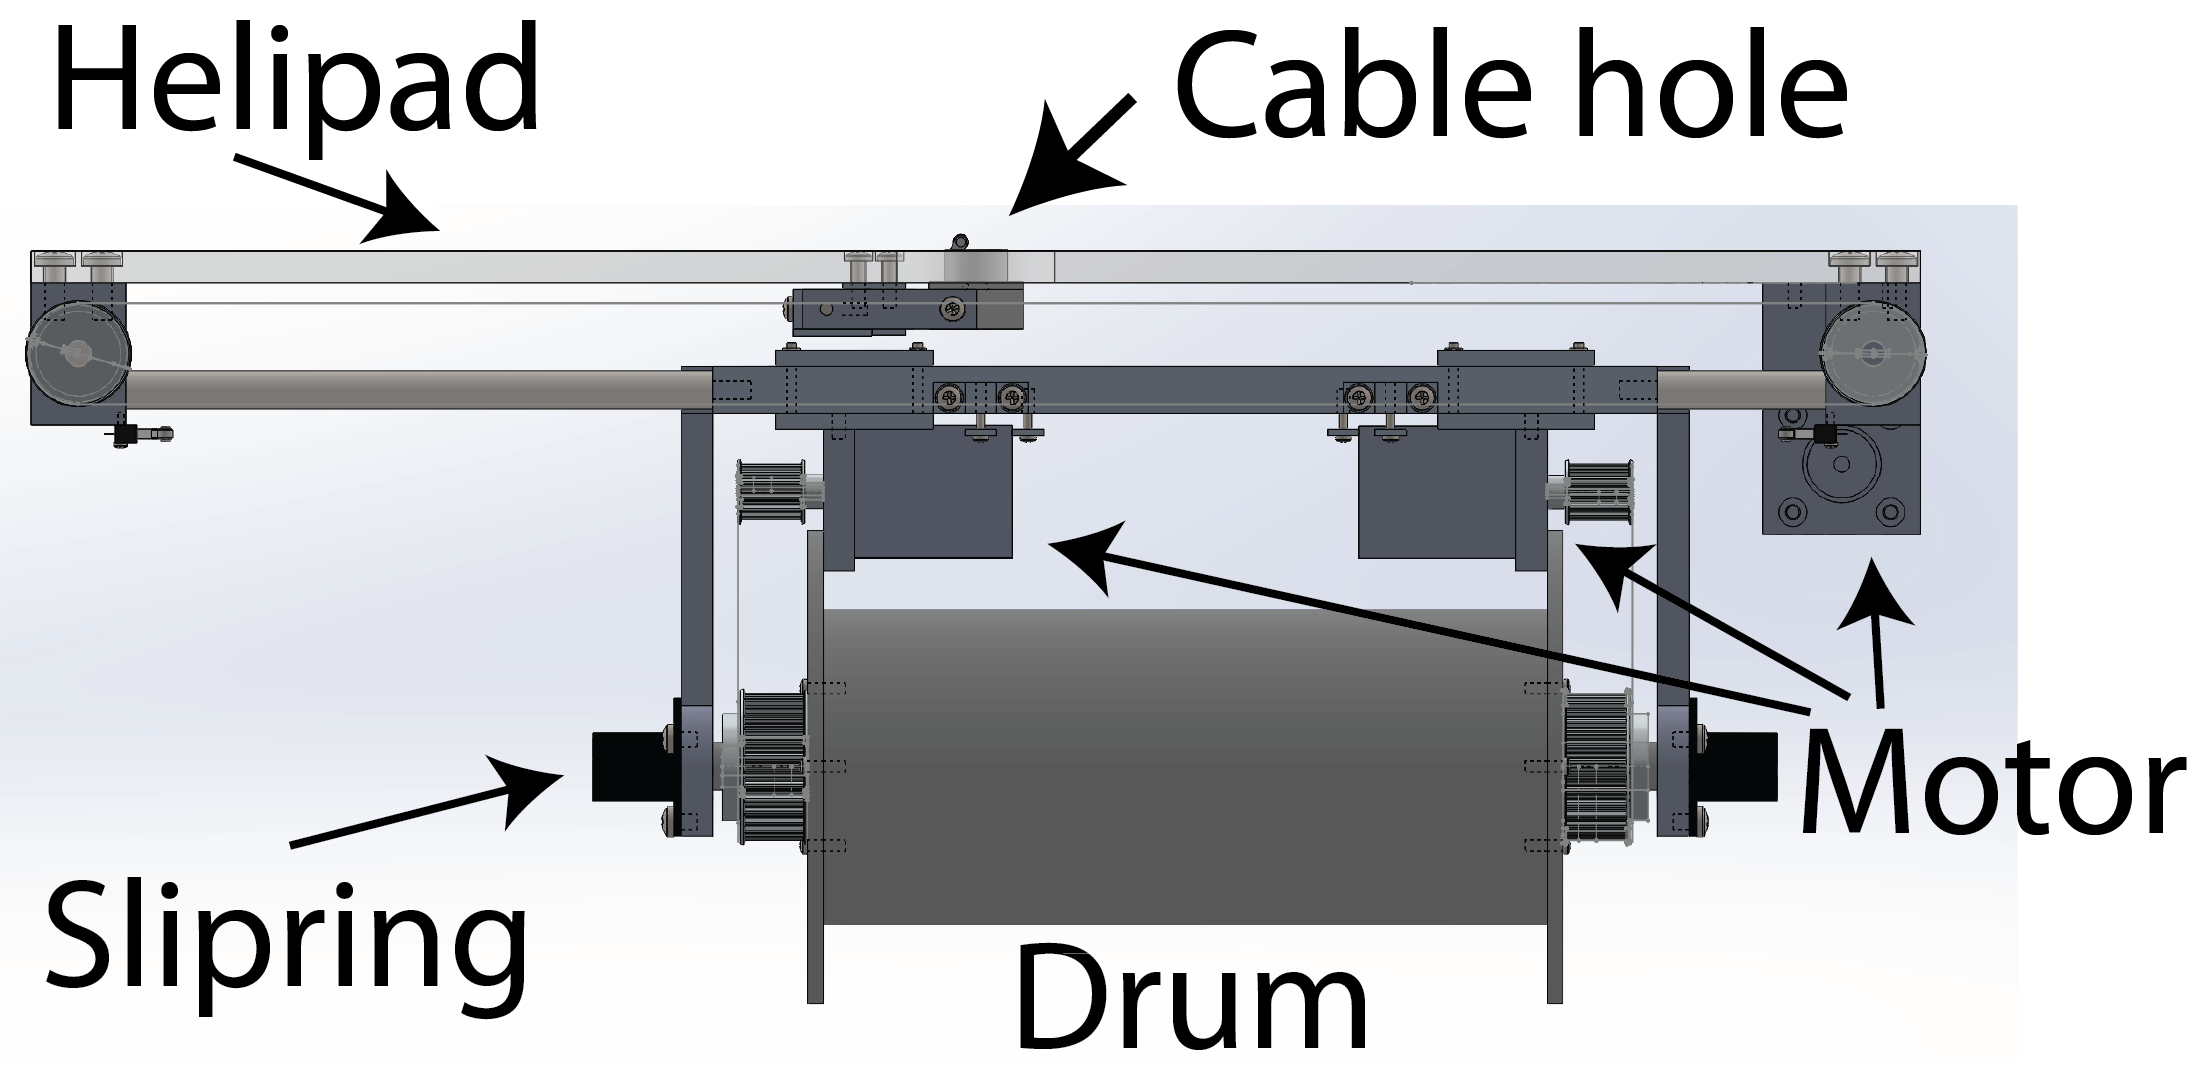
\includegraphics[scale=0.75]{graphics/cad/cable-drum.png}
\caption[Cable drum design]{Cable drum design. The drum can rotate to winch in/out the cable, and also move from side-to-side to assure smooth windings.}
\label{fig:cable-drum}
\end{figure}

\noindent
With all wire winded in and the UAV on maximum throttle there is assumed to be 500W running through the cable with a electrical loss at around 120 Watt, which is transformed into heat. 120 Watt of heat will give rise to heating up the cable drum. This is a known cause of electrical fire, when a cable drum gets too hot and melts. Therefore a series of pretests where performed to address how big a problem this would be, and to incorporate the result in the design of the system. The test and results are described in next chapter.



\subsection{The Simple Winch}
Sometimes simple is better. The simple design have a motorized toothed wheel and an encoder wheel pushing the cable against the wheels. The encoder wheel turns only when the cable is moving, and the slip is minimal making it a very robust feedback for the motor controller. The encoder wheel is pushing the cable toward the motor wheel with a spring, that assures small imperfections in the cable does not make it slip. two simple screws adjust the spring tension. For storing the cable a box underneath collects the cable.

\begin{figure}[H]
\centering
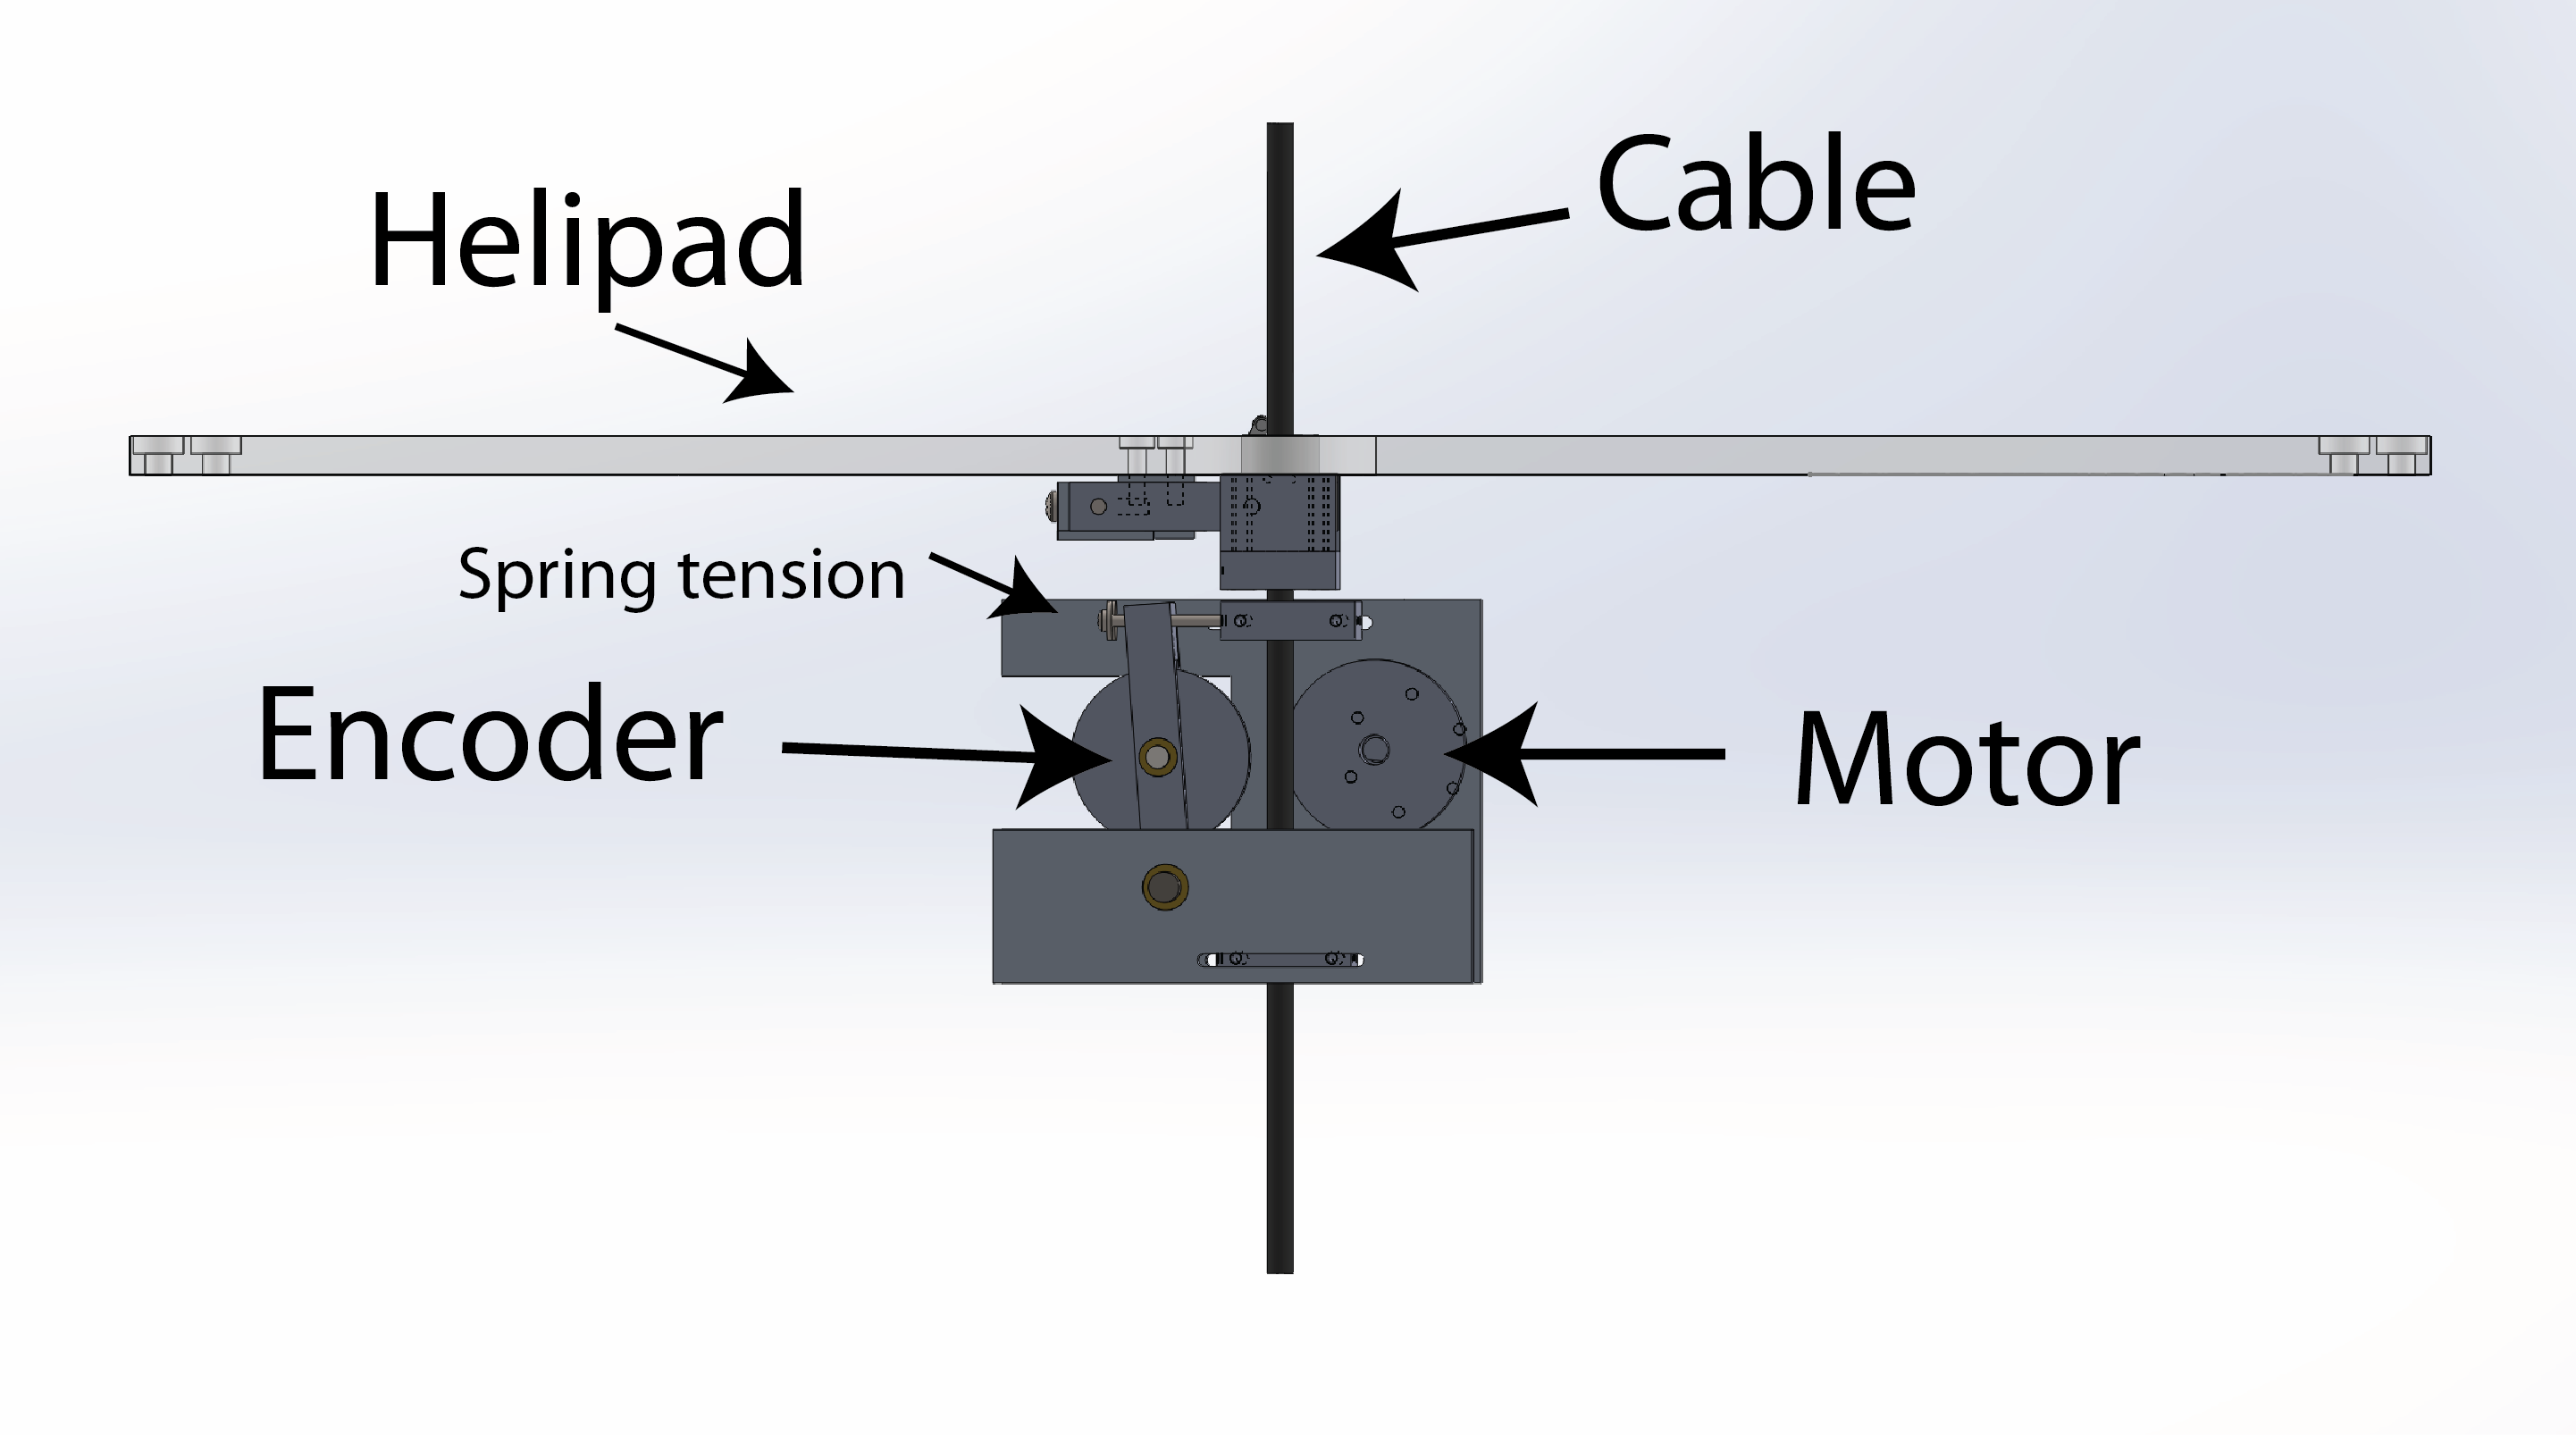
\includegraphics[scale=0.75]{graphics/cad/winch.png}
\caption[The Simple Winch]{The Simple Winch only has one motor and an encoder wheel pushing the cable towards the motor wheel. Two springs adjust the tension.}
\label{fig:winch}
\end{figure}

\subsection{Summary}
Both concepts are mature enough to be prototyped and tested, but due to the time frame of this work there is only time for manufacturing and testing one design. Based on the lower mechanical complexity of the simple winch, the simple winch is the chosen design.    


\section{Cable Connection point on the UAV}
Connecting the cable to the UAV have several issues to address. First a 3-axes measurement device is needed to measure how much the cable tension is and in tree directions - $x$, $y$, and $z$ directions. The load cells used is of same type as in measuring the horizontal angle in section \ref{sec:horizontalAnglePrototype} on page \pageref{sec:horizontalAnglePrototype}. In $z$-direction the maximal force applied to the load cell is the UAVs lifting capability on approximately 3kg\todo{Citer adriana}. Hence the choice of load cell is a 5kg load cell.\\
\noindent
In $x$- and $y$-direction the force applied by the cable or the UAV is not expected to exceed $0.5$kg, thus two smaller $0.78$kg load cell is used to measure the $x$- and $y$-directional force. 

\begin{figure}[hbtp]
\centering
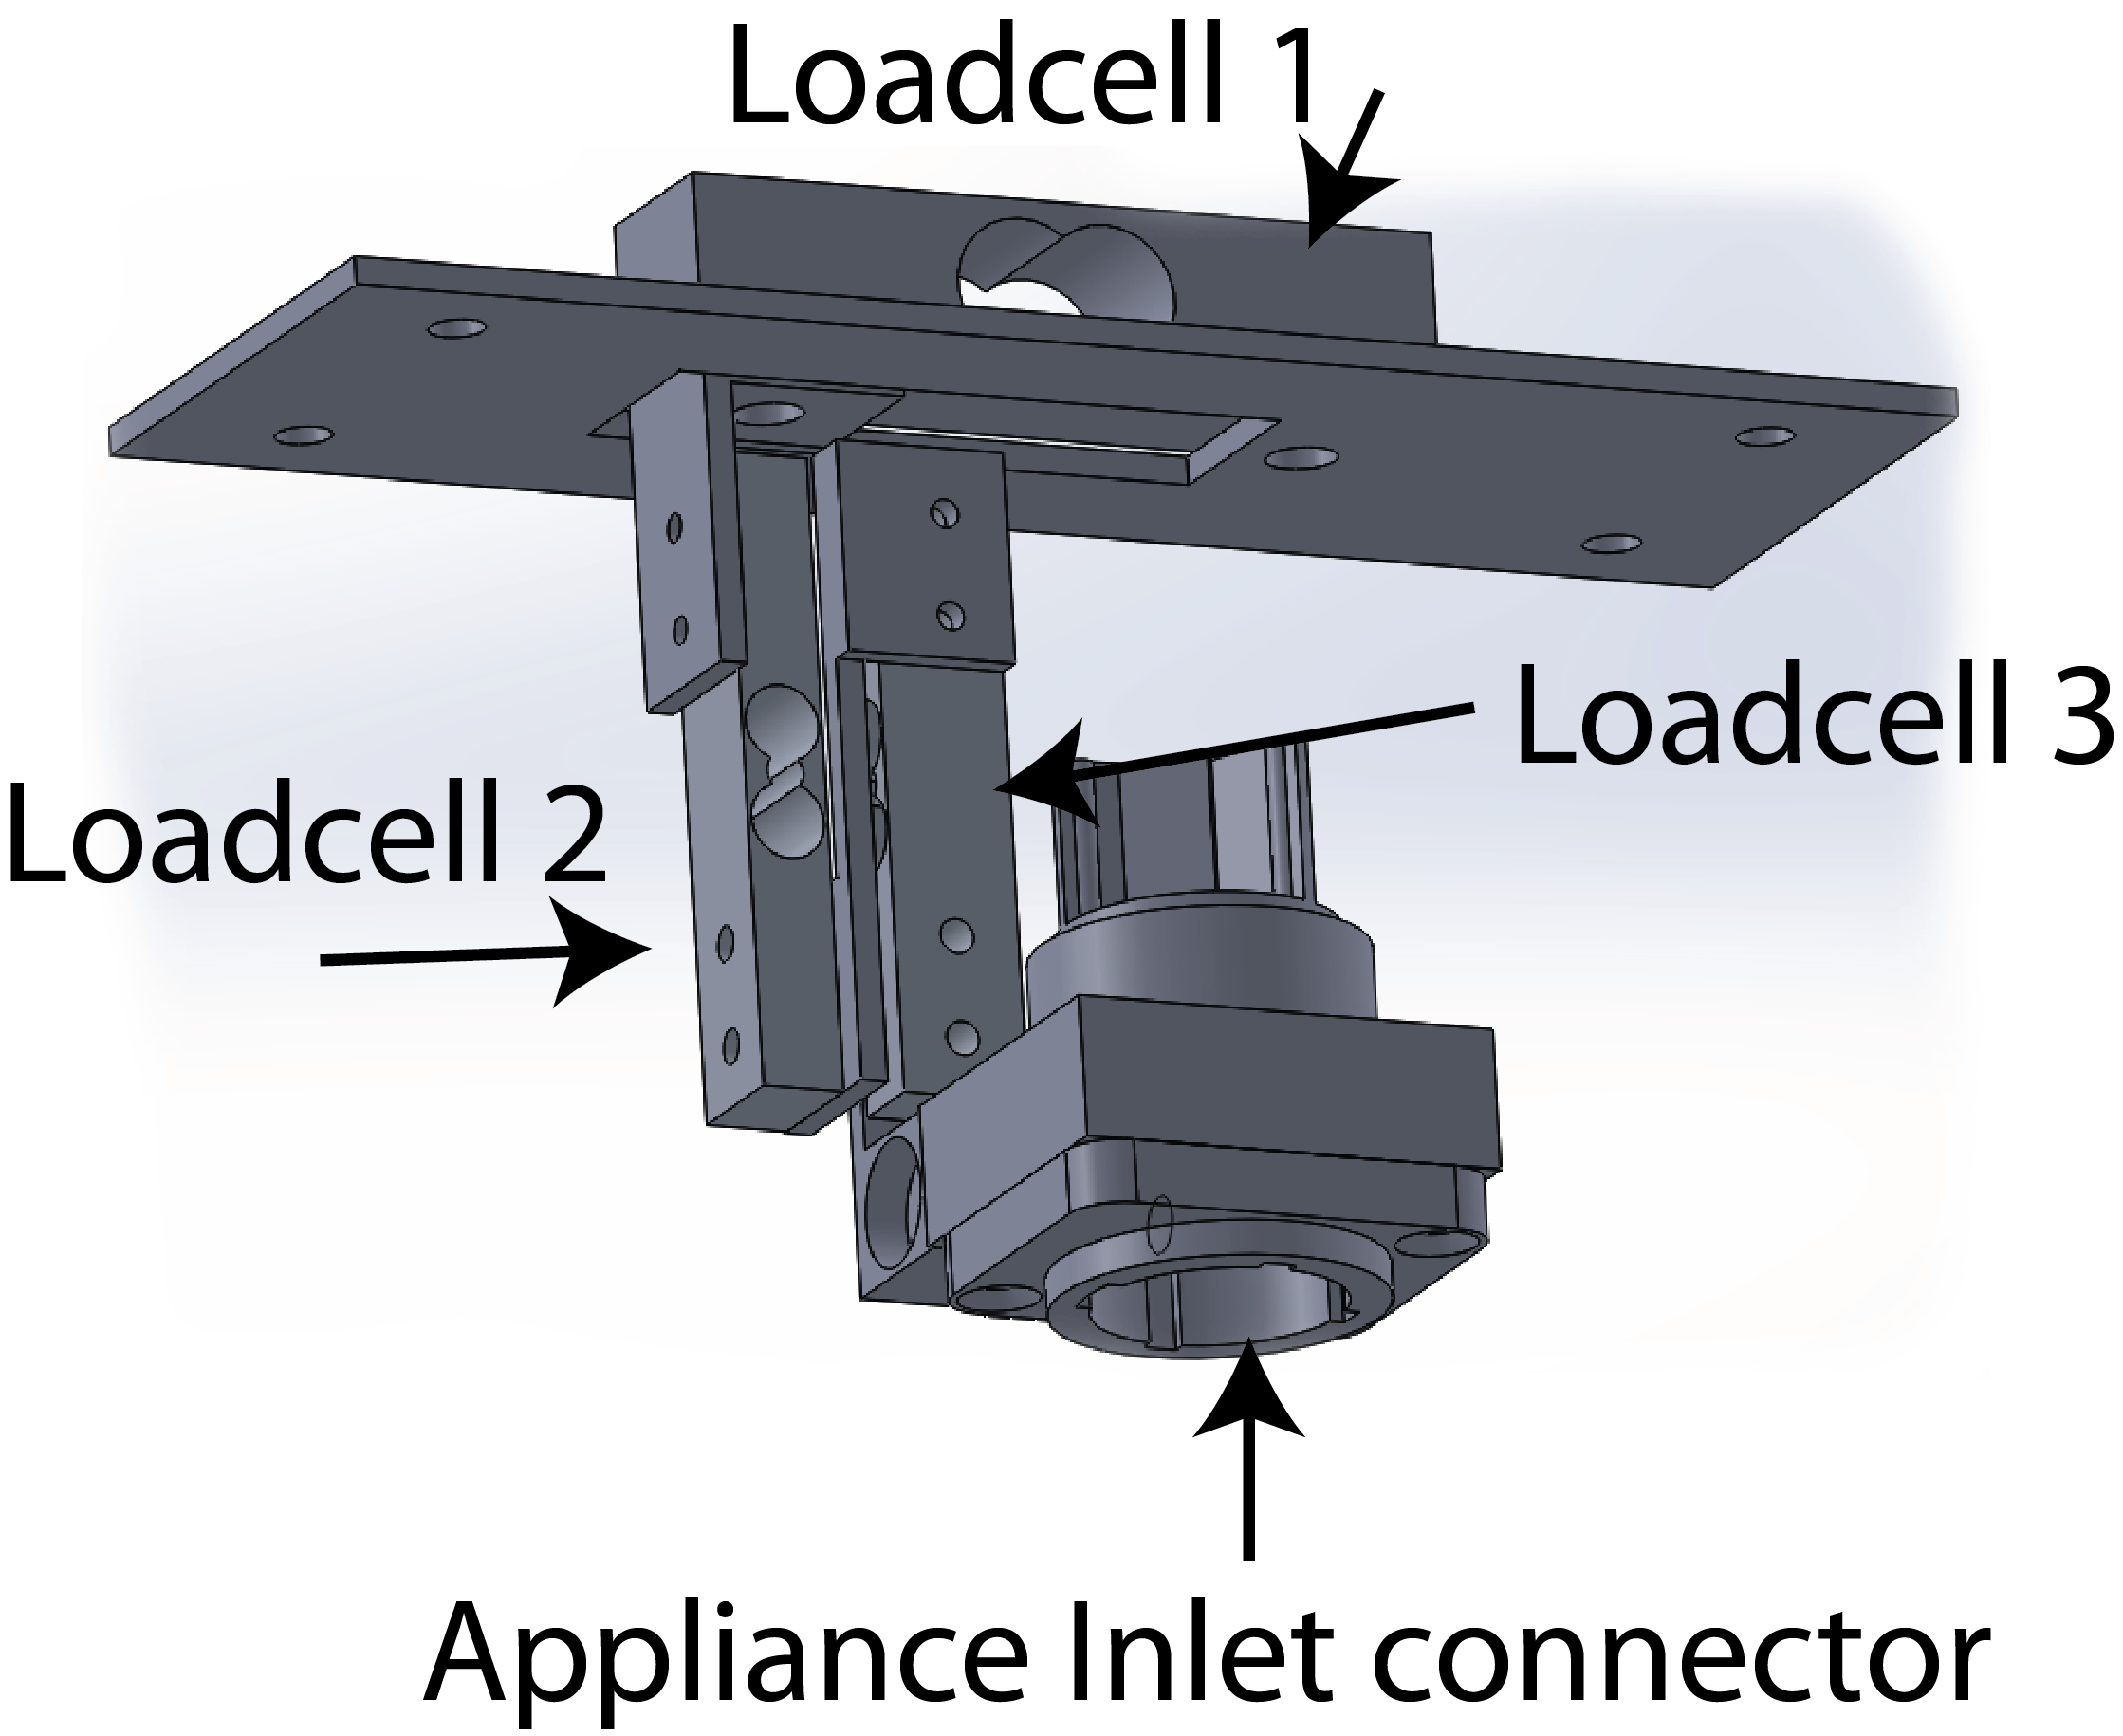
\includegraphics[scale=0.5]{graphics/cad/hexa.png}
\caption{3-axes measuring device for the UAV with appliance inlet connector.}
\end{figure}


\noindent
Second an appliance inlet connector for easy plug-in and unplug is wanted. The connector must be capable to withstand the weight of the cable and the force applied of the UAV. 

\begin{figure}[hbtp]
\centering
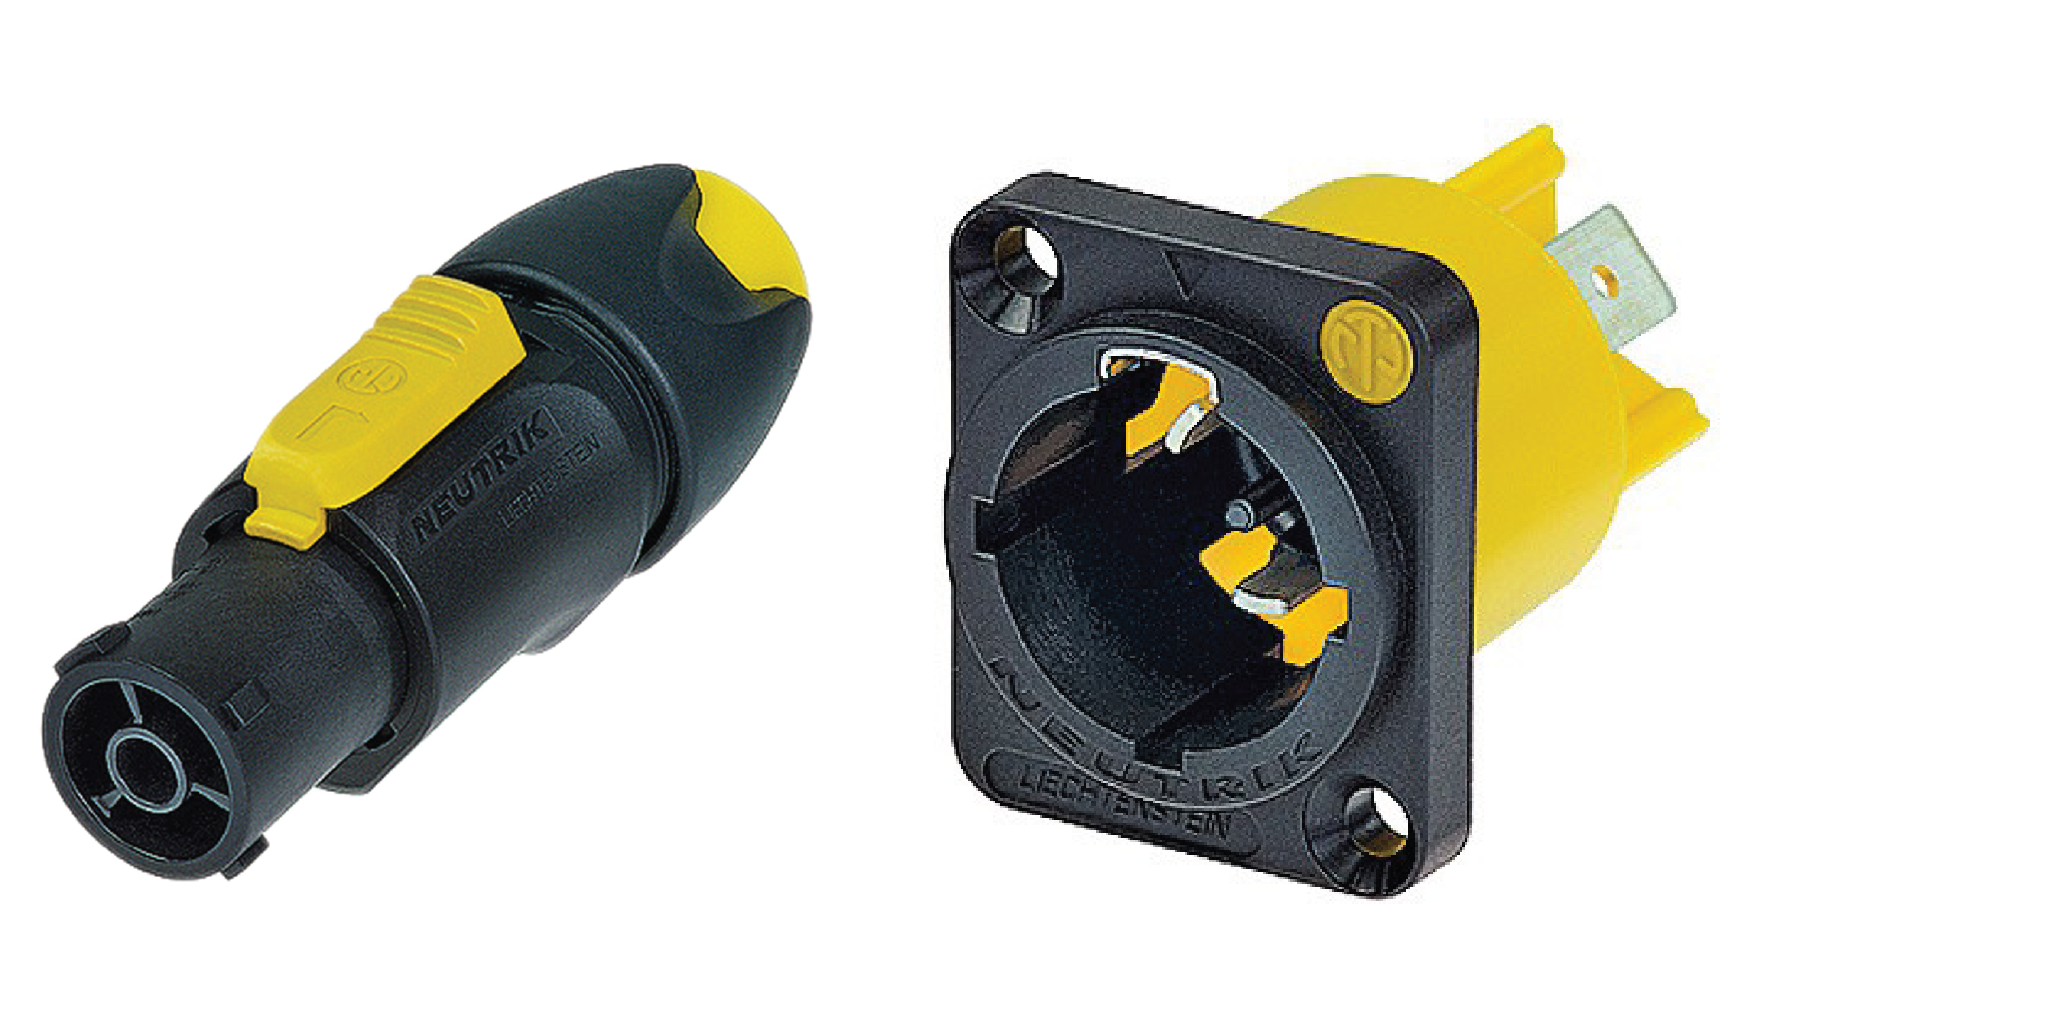
\includegraphics[scale=1]{graphics/Neutrix-True-One.png}
\caption{Neutrix True One appliance connector system.}
\end{figure}



\section{Electrical Design}
From an electrical view there are two separate systems, Flight Control System on the UAV and Ground Control Station. The system reading the sensor data on the Ground Control Station has to feed the UAV with the measured data hence the UAVs position controller is running on the UAV. 
\todo{Introducer 12V/75V system}

\subsection{Ground Station}
The ground station sends data to the UAV system and decides weather to roll cable in or out based on the wanted position. The control of feeding the cable is done by comparing the load on the UAV system to what is expected by the weight of the rolled out amount of cable. If the load is higher then expected more cable are rolled out and vice versa.  
\begin{figure}[hbtp]
\centering
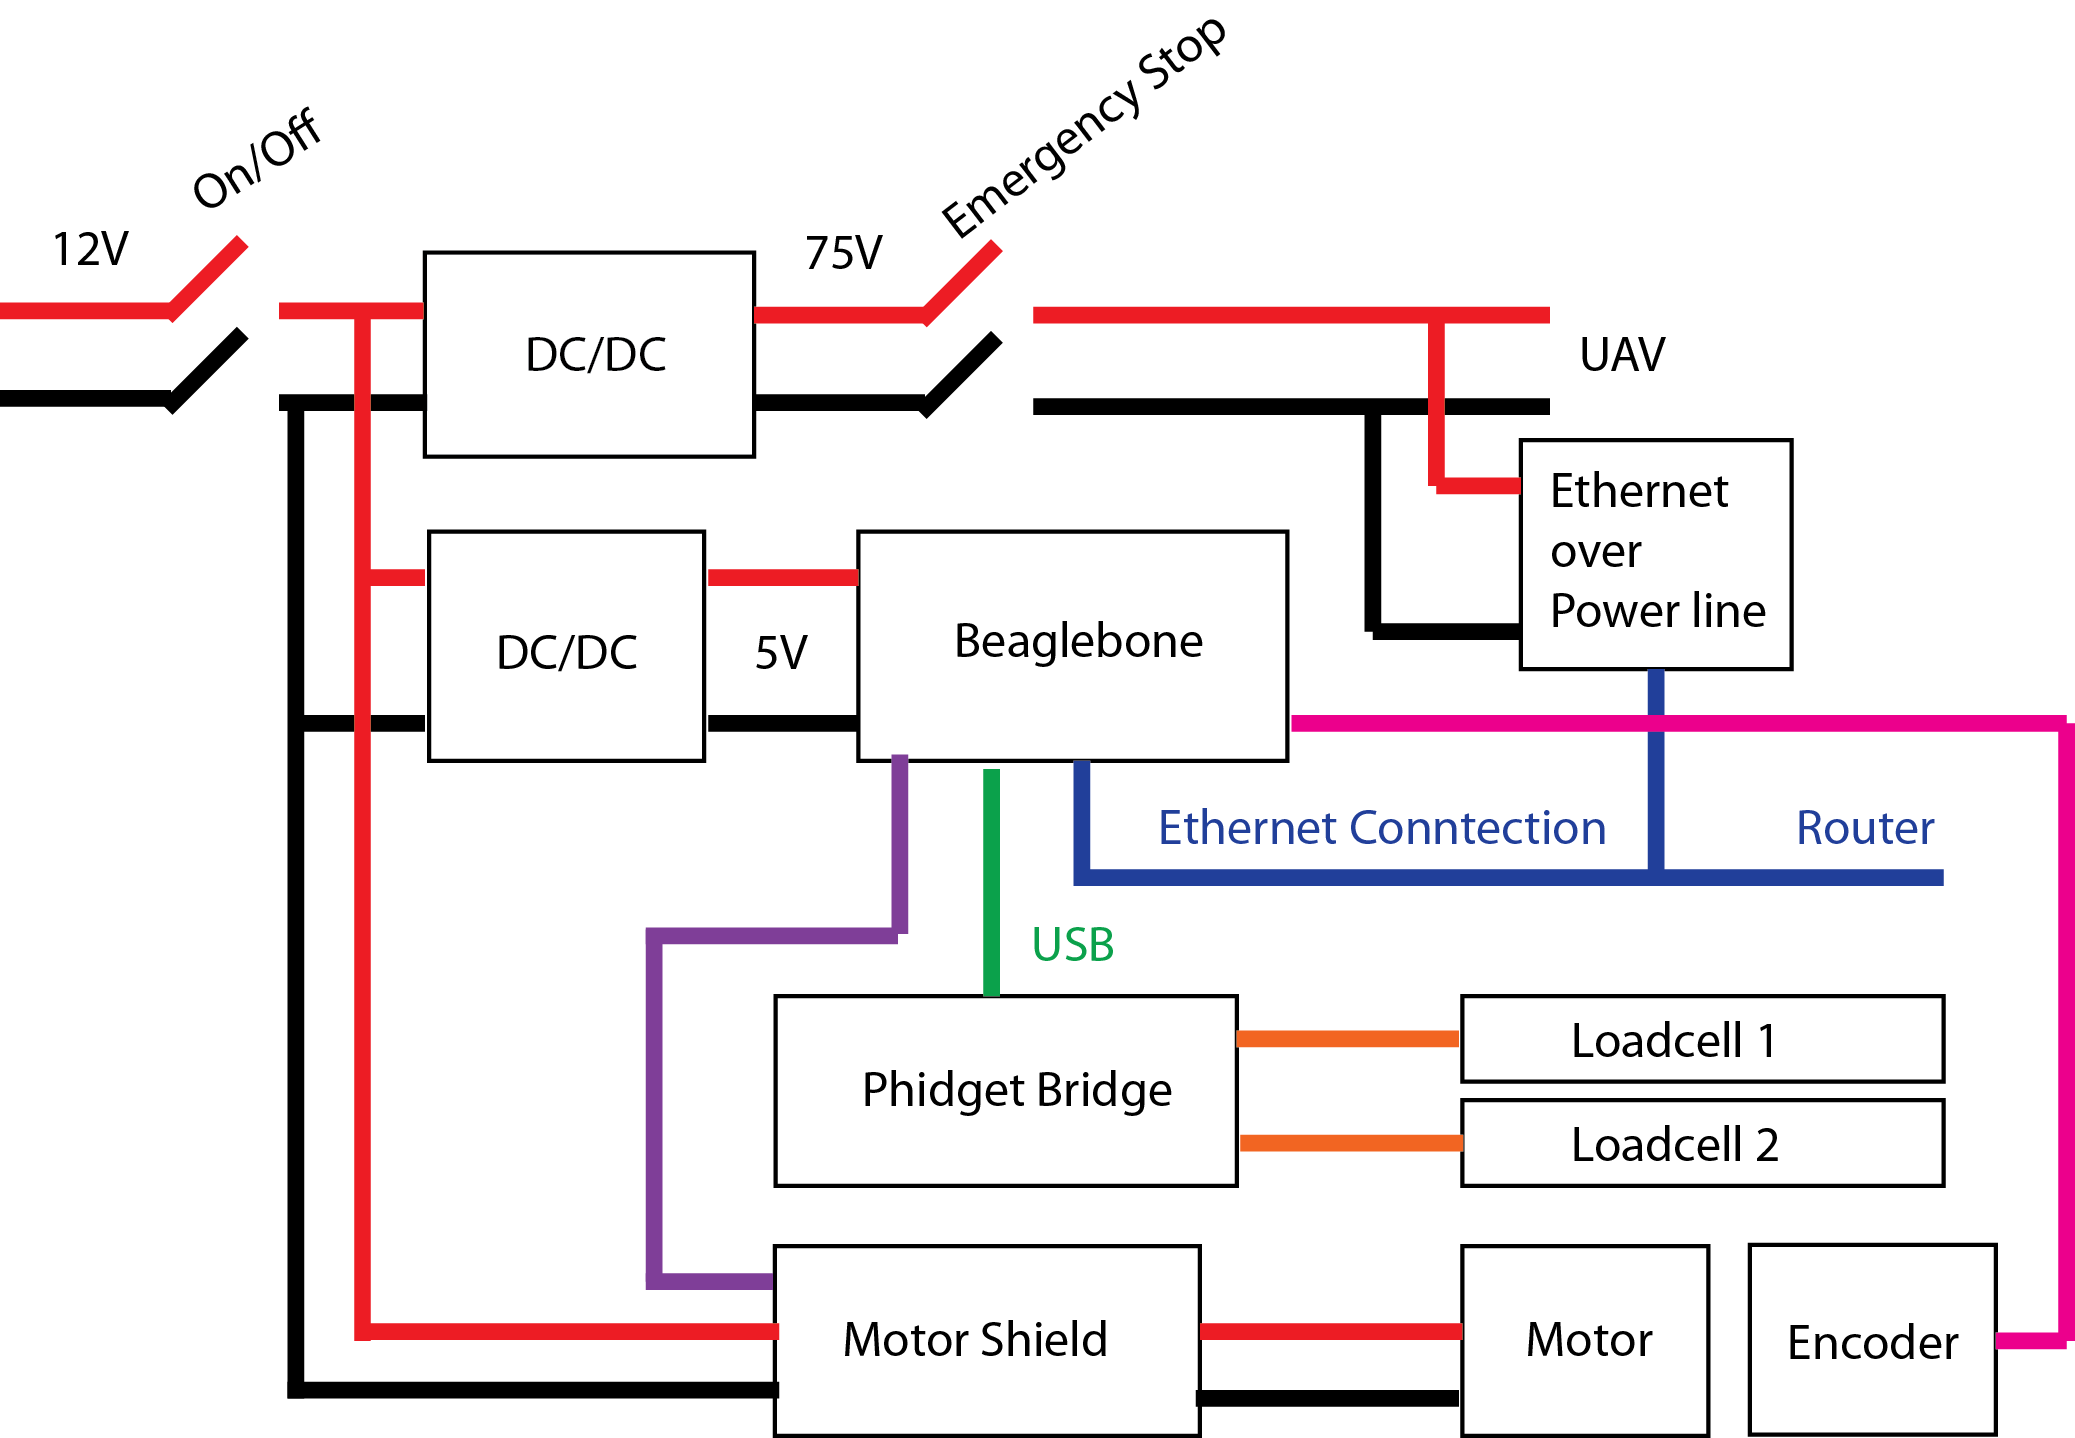
\includegraphics[scale=0.75]{graphics/GCS-eltectrical-overview.png}
\caption{Ground Station electrical overview.}
\end{figure}


\subsection{UAV System}
The system on the UAV measures a 3-axes load cell connected to a Phigets Bridge. The Phidget Bridge are interfaced via a Beaglebone Black.  

\begin{figure}[hbtp]
\centering
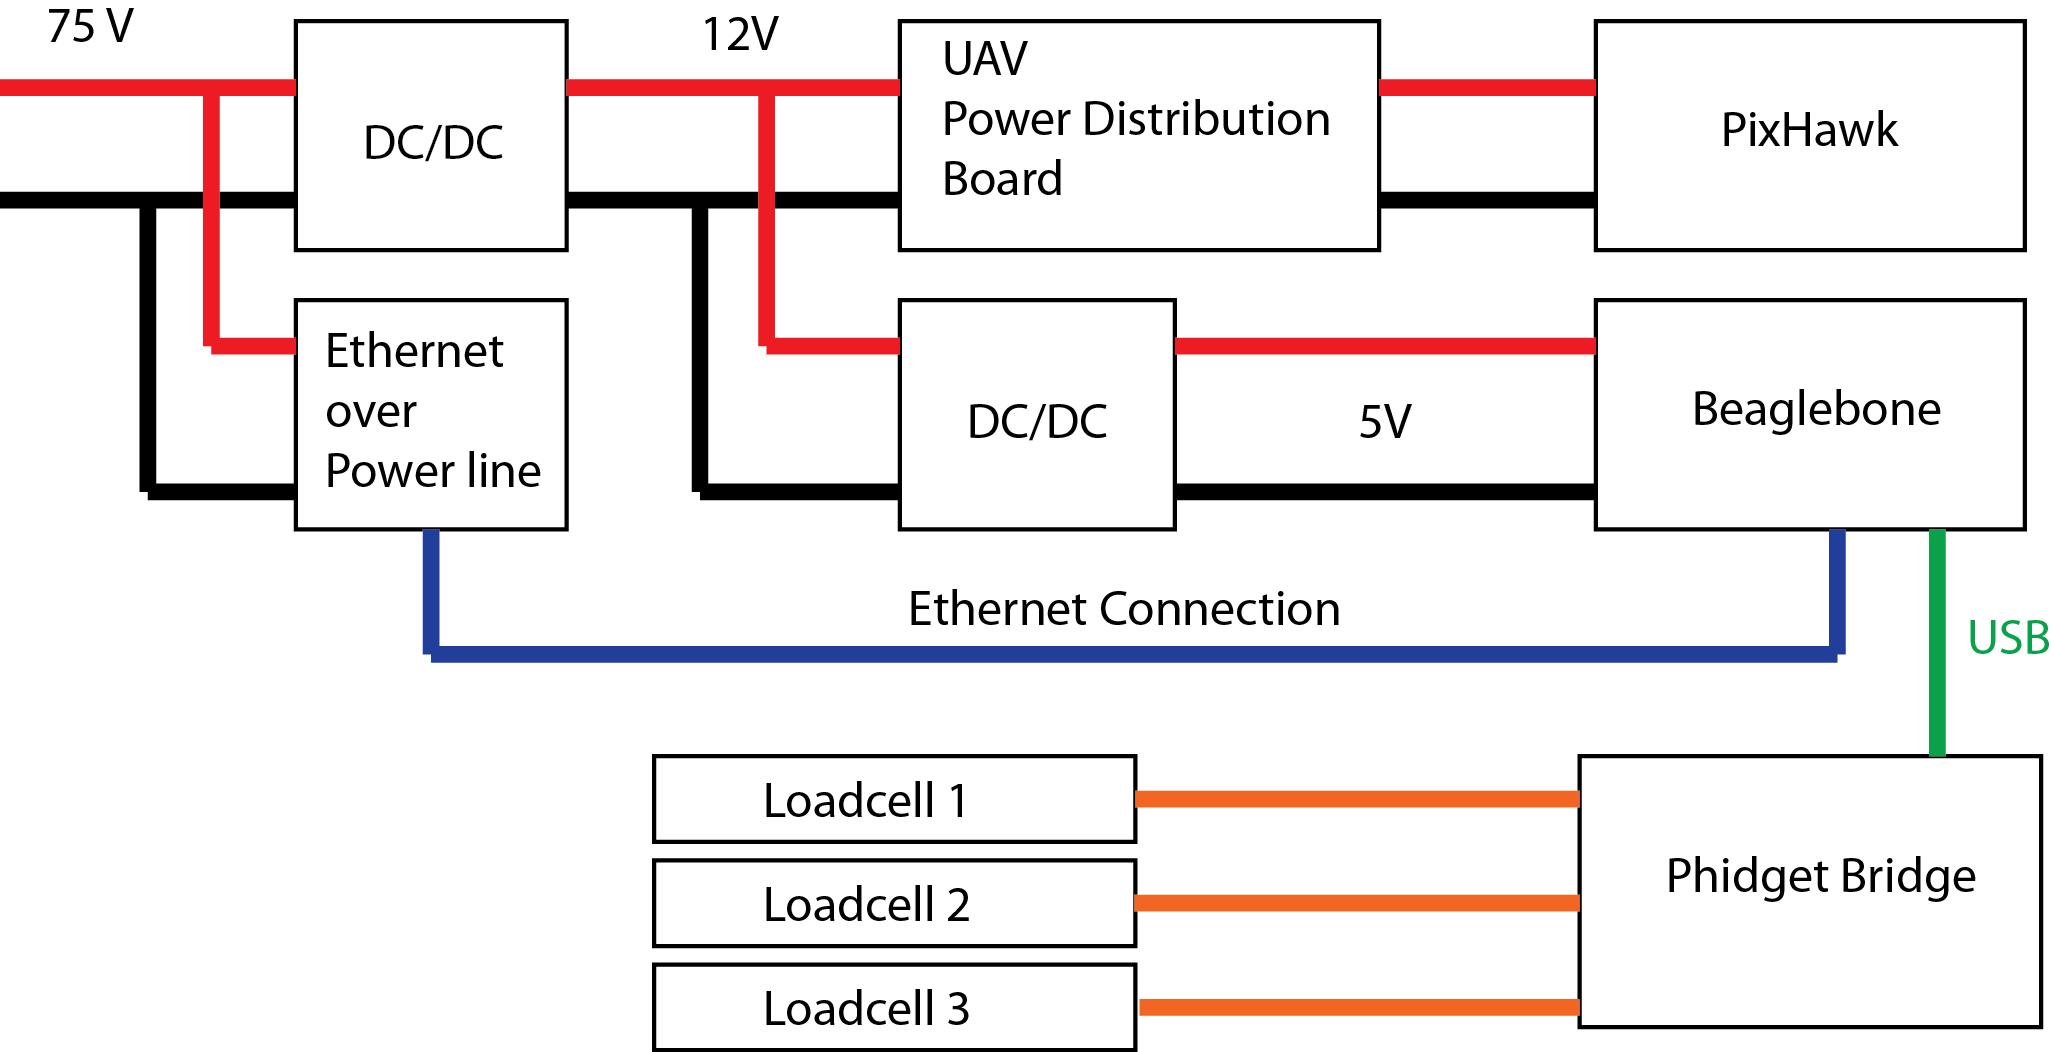
\includegraphics[scale=0.75]{graphics/UAV-electrical-system.png}
\caption{UAV electrical overview.}
\end{figure}



\subsection{Data Connection using Ethernet over Power line}
To connect the UAV to the Ground Station an Ethernet over power line system is used. Ethernet over power line operate by adding a modulated carrier to the wiring system, intended to work on 110-230 volt AC with frequencies in 50-60 Hertz. The AV500 Nano\footnote{Model number: TL-PA411KIT.} system from TP-Link supports speeds up to 500Mbps and works without any configuration needed. Stripping the housing from the electronic and soldering two wires on to parallel connect the component to the 75 volt system. 

\begin{figure}[hbtp]
\centering
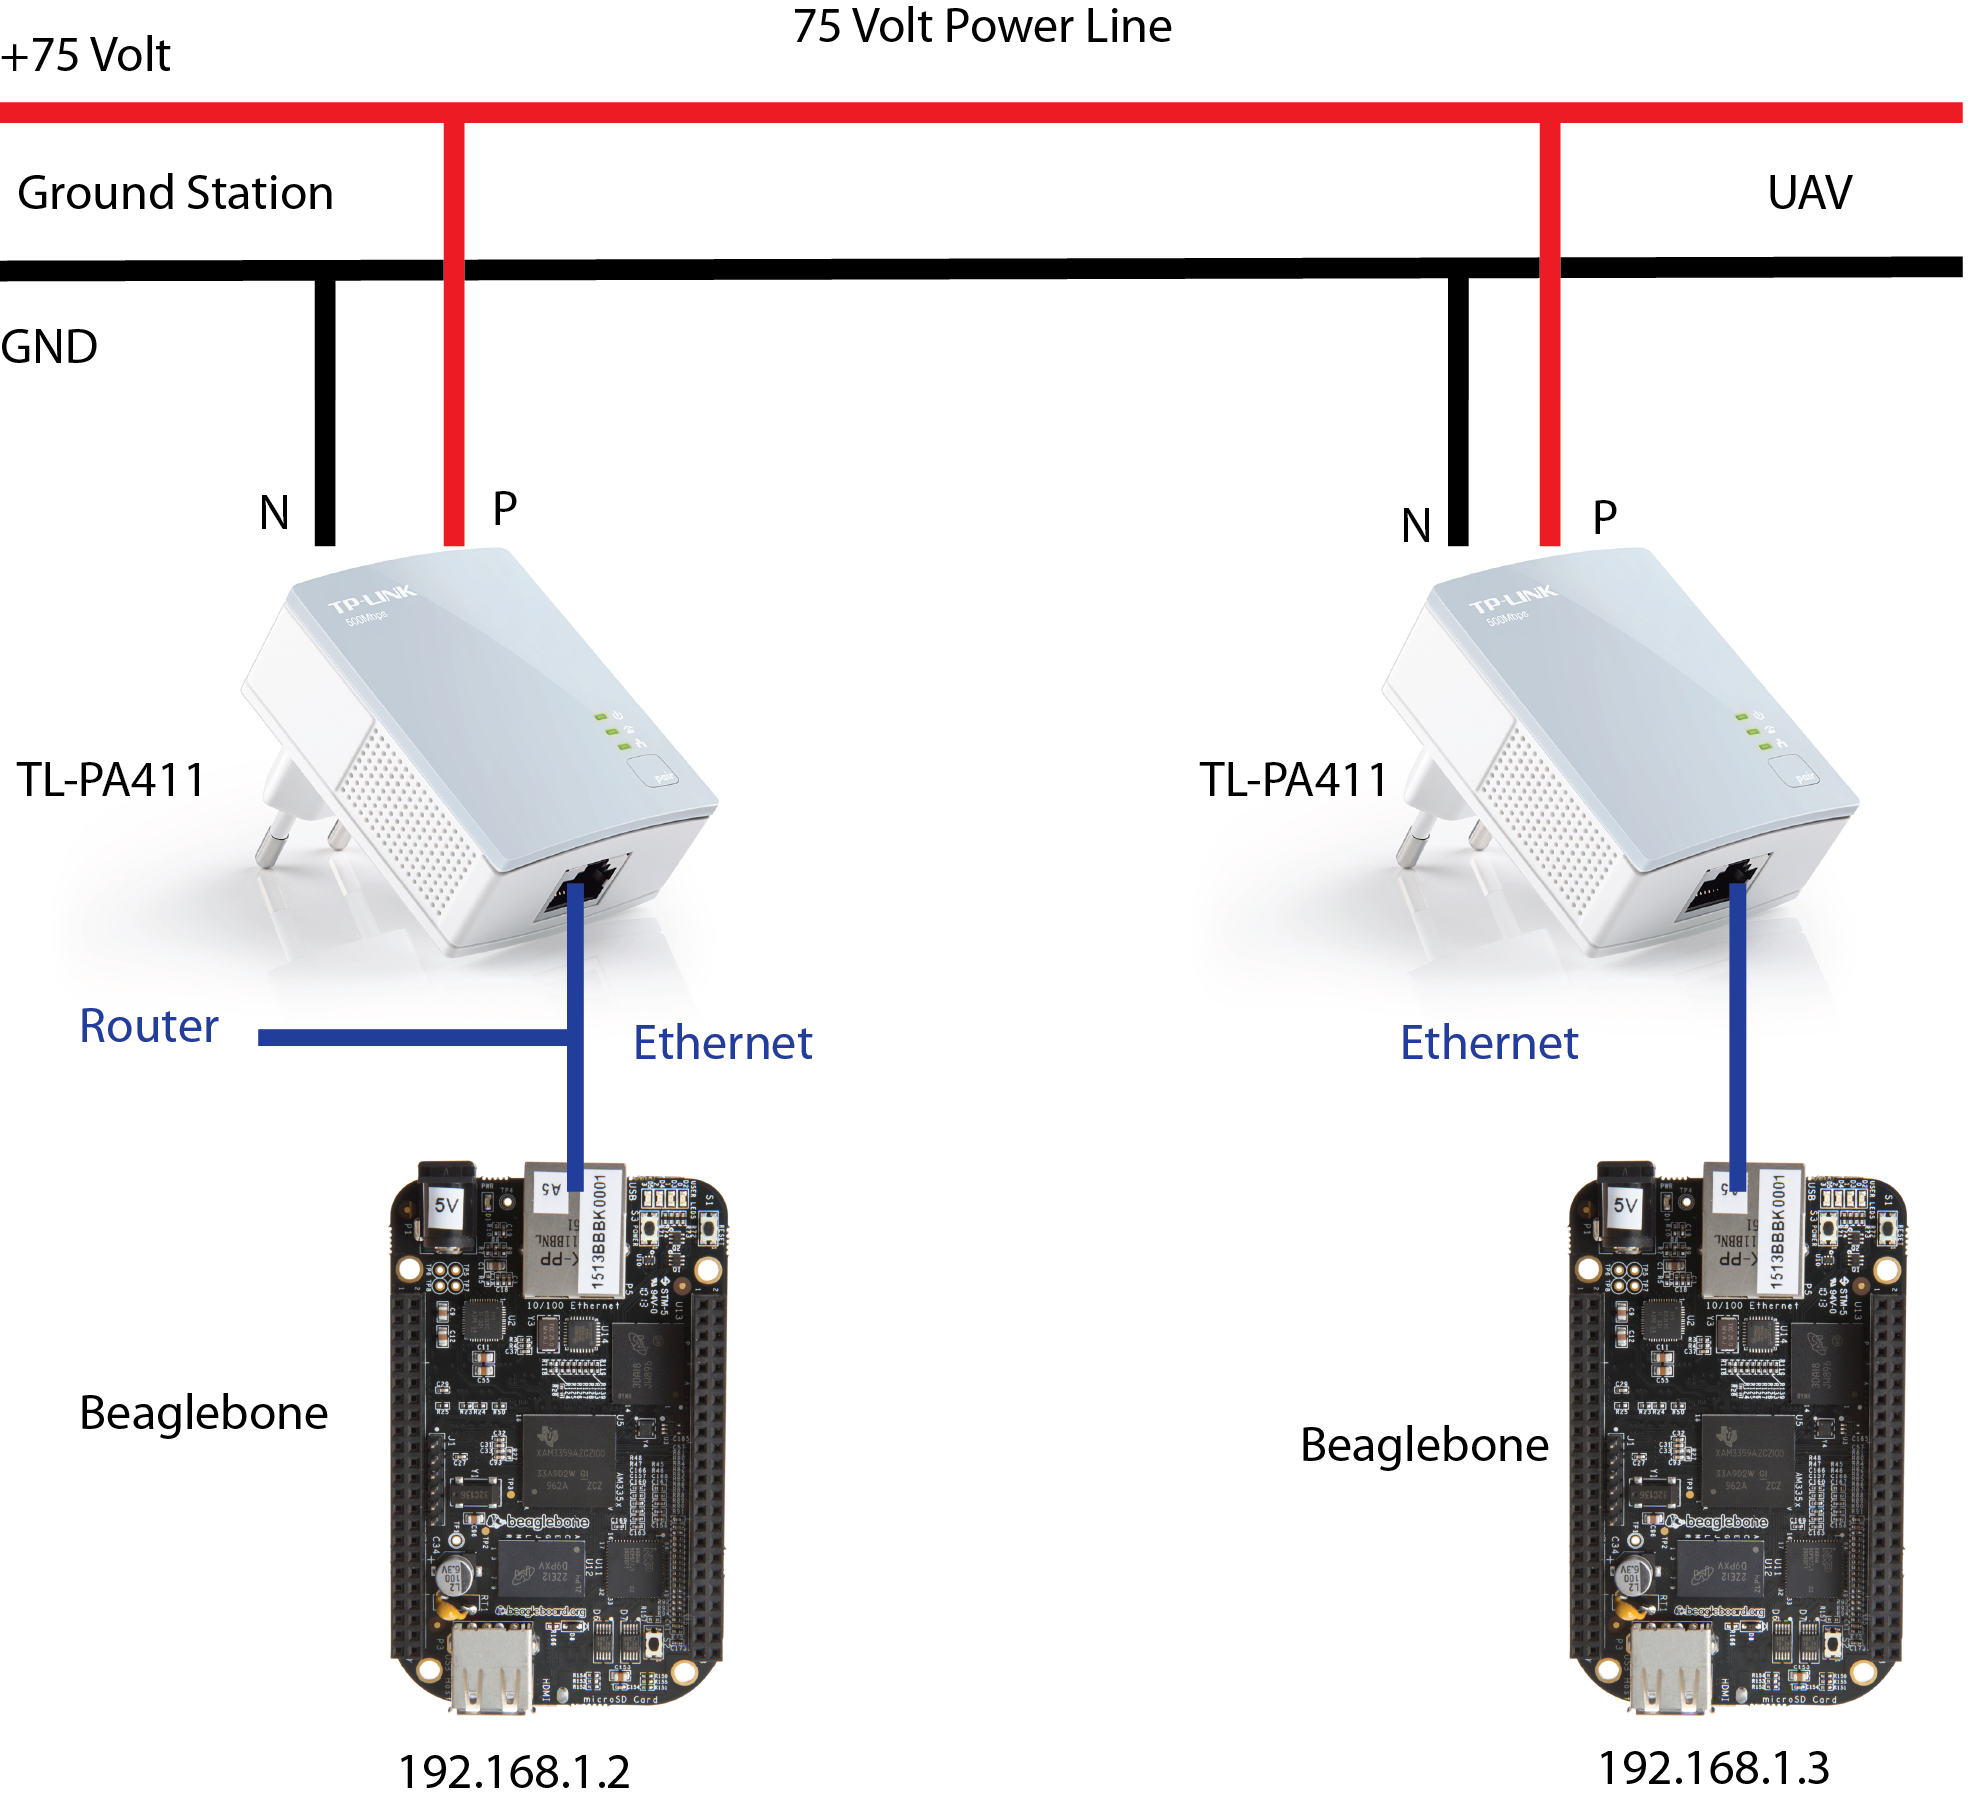
\includegraphics[scale=0.75]{graphics/EthernetLink.png}
\caption[Ethernet over power line setup]{Ethernet over power line setup. Two TL-PA411 is connected to the 75 volt powerline creating an Ethernet over power line connection to the UAV.}
\label{fig:Networking}
\end{figure}



\section{Software Design}
All software for measuring and controlling is implemented in the real-time software framework Robot Hardware Daemon, RHD. RHD is the real-time hardware abstraction layer for the Mobotware platform, developed at the deparment of Automation and Control at DTU. RHD is a plugin-based platform that allows easy integration with sensors and actuators. RHD creates a synchronized database with read/write variables that can be shared between plugins and/or accessed by other software applications.

\subsection{Ground Control Station}
The objective of the Ground Control station software is to measure the horizontal force, fetch steering reference signals from joystick or other controller, control the cable winch, and make the calculated control signals available in the variable database. On figure \ref{fig:GCS-software-overview} a graphical overview of the plugin structure shows the periodic run sequence and plugin variable dependency relationship. The speed variables are created in the plugin tcuav, and not the joycontrol hence the joycontrol module estimates the steering method by variables available. This also mean the initialization of joystick must be performed after initialization of tcuav. 
\todo{Fortæl om GPIO+Encoder}
\begin{figure}[hbtp]
\centering
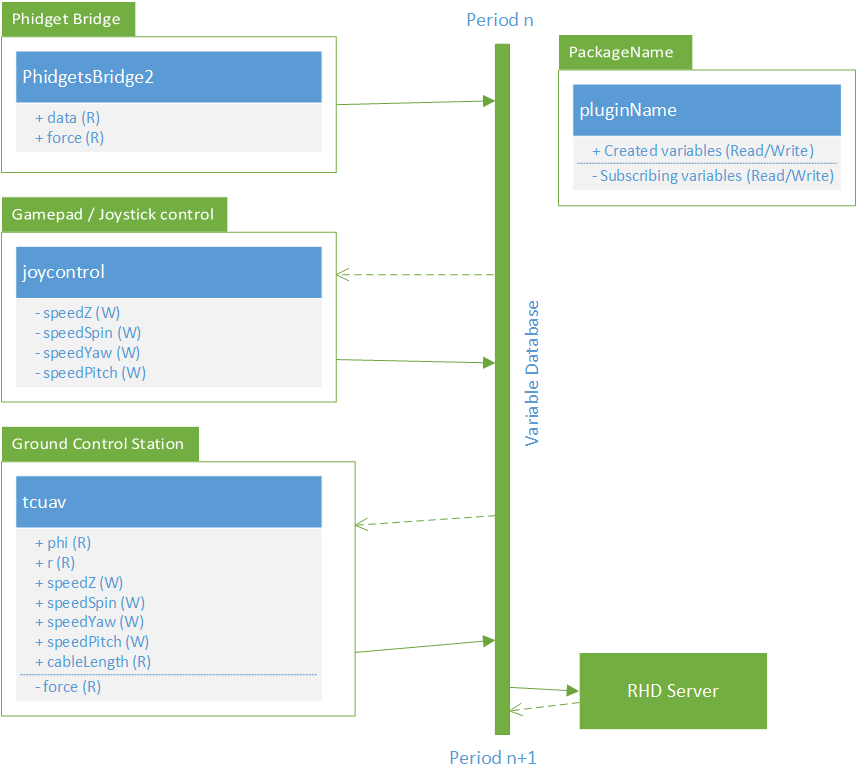
\includegraphics[scale=0.8]{graphics/Visio/GCS-software-overview.png}
\caption[Ground Control Station software overview]{Ground Control Station software overview based on the RHD plugin structure showing plugin sequence for one sample period.}
\label{fig:GCS-software-overview}
\end{figure}




\subsection{Flight Control System}
The objective of the Flight Control System is to measure the force from the 3-axes load cell system, establish a link connection to Ground Control Station and fetch control variables, and make control variables available to the PixHawk(UAV Flight Controller).


\begin{figure}[hbtp]
\centering
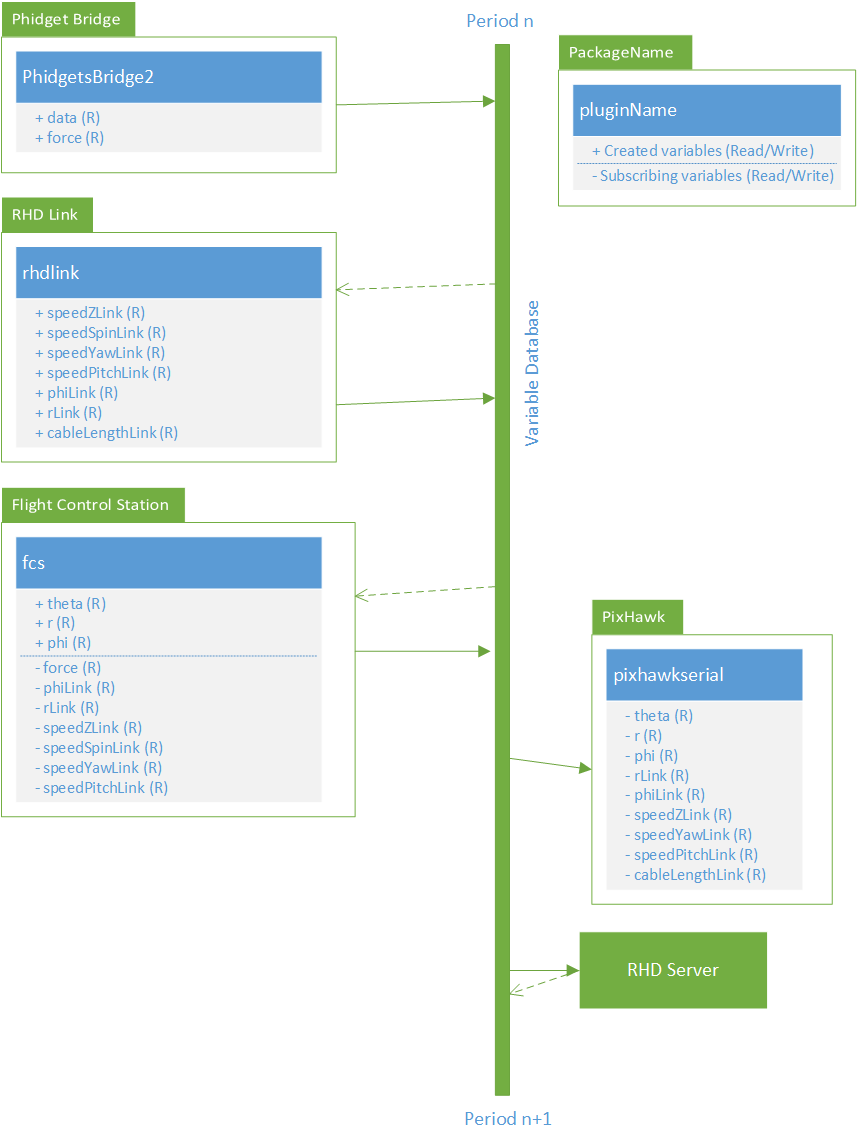
\includegraphics[scale=0.8]{graphics/Visio/FCS-software-overview.png}
\caption[Flight Control System software overview]{Flight Control System software overview based on RHD plugin structure showing plugin sequence for one sample period.}
\end{figure}
